%!Mode::"UTF-8"
\documentclass[12pt]{article}

% 页面设置
\usepackage{geometry}
\geometry{left=2.5cm, right=2.5cm, top=2.5cm, bottom=2.5cm}
\usepackage{graphicx}
\usepackage{ctex}
\usepackage{fontspec}
\usepackage{setspace}

% 代码设置
\usepackage{listings}
\usepackage{color}
\setmonofont{Consolas}
\definecolor{listing}{gray}{0.97}
\lstset{
	backgroundcolor=\color{listing},
	basicstyle=\footnotesize,
	numbers=left,
	numberstyle=\footnotesize,
	stepnumber=1,
	aboveskip={0.5\baselineskip},
	belowskip={0.5\baselineskip},
	columns=fullflexible,
	breaklines=true,
	breakatwhitespace=true,
	frame=single,
	basicstyle=\ttfamily,
	numberstyle=\ttfamily,
	tabsize=2
}

% 字体设置
\setmainfont{Times New Roman}
\setCJKmainfont{SimSun}
\setCJKsansfont{SimHei}

% 表格设置
\usepackage{makecell}
\newcommand{\addcell}[2][4]{\makecell{\zihao{#1}\textsf{#2}}}
\usepackage{titlesec}
\usepackage{booktabs}
\usepackage{tabularx}

% 设置图注、表注
\usepackage{caption}
\usepackage{bicaption}
\captionsetup{labelsep=quad, font={small, bf}, skip=2pt}
\DeclareCaptionOption{english}[]{
    \renewcommand\figurename{Fig.}
    \renewcommand\tablename{Table}
}
\captionsetup[bi-second]{english}

% 设置页眉
\usepackage{fancyhdr}
\pagestyle{fancy}
\fancypagestyle{preContent}{
    \fancyhead[L]{\zihao{-5} 物理化学实验}
    \fancyhead[C]{\zihao{-5} 实验五\ \ 蔗糖的转化}
    \fancyhead[R]{\zihao{-5} 1800011828\ 王宇哲}
}
\pagestyle{preContent}

%	设置首页页眉页脚
\fancypagestyle{plain}{
	\fancyhead[L]{\zihao{-5} 物理化学实验}
	\fancyhead[C]{\zihao{-5} 实验五\ \ 蔗糖的转化}
	\fancyhead[R]{\zihao{-5} 1800011828\ 王宇哲}
	\cfoot{}
}

% 设置标题格式
\titleformat*{\section}{\zihao{4}\sffamily}
\titleformat*{\subsection}{\zihao{-4}\sffamily}
\titleformat*{\subsubsection}{\zihao{-4}\sffamily}
\titlespacing*{\section}{0pt}{10pt}{10pt}
\titlespacing*{\subsection}{0pt}{10pt}{5pt}
\titlespacing*{\subsubsection}{0pt}{10pt}{5pt}

% 设置引用格式
\usepackage[super,round,comma,compress]{natbib}

\usepackage{amsmath}
\usepackage{amssymb}

%设置封面
\begin{document}
    % 标题页
    \begin{titlepage}
    	% 页眉
    	\thispagestyle{plain}
        % 图片
        \begin{figure}[h]
            \centering
            \includegraphics{pku.png}
        \end{figure}
        \vspace{24pt}
        % 标题
        \centerline{\zihao{-0} \textsf{物理化学实验报告}}
        \vspace{40pt} % 空行
        \begin{center}
            \begin{tabular}{cp{6.5 cm}}
                % 题目
                \addcell[2]{题目:\ } & \addcell[2]{蔗糖的转化} \\
                \cline{2-2}
            \end{tabular}
        \end{center}
        \vspace{20pt} % 空行
        \begin{center}
            \doublespacing
            \begin{tabular}{cp{5cm}}
                % 姓名
                \addcell{姓\phantom{空格}名:\ } & \addcell{王宇哲} \\
                \cline{2-2}
                % 学号
                \addcell{学\phantom{空格}号:\ } & \addcell{1800011828}\\
                \cline{2-2}
                % 组别
                \addcell{组\phantom{空格}别:\ } & \addcell{11组} \\
                \cline{2-2}
                % 实验日期
                \addcell{实验日期:\ } & \addcell{2020.11.11}\\
                \cline{2-2}
                % 室温
                \addcell{室\phantom{空格}温:\ } & \addcell{296.45\ K}\\
                \cline{2-2}
                % 大气压强
                \addcell{大气压强:\ } & \addcell{102.81\ kPa}\\
                \cline{2-2}
            \end{tabular}
            \begin{tabular*}{\textwidth}{c}
                \\ % 这是空行
                \\ % 这是空行
                \\ % 这是空行
                \\ % 这是空行
                \hline % 分割线
            \end{tabular*}
        \end{center}
        % 摘要
        \textsf{摘\ \ 要}\ \ 本实验使用目视旋光仪测定蔗糖转化过程中体系旋光度的变化,验证了蔗糖转化反应对蔗糖是一级反应,作出了不同盐酸浓度下混合液$\alpha_{t}-t$图和${\rm lg}(\alpha_{t}-\alpha_{\infty})-t$图,测定了加入盐酸浓度分别为$2.12\ \ {\rm M}$、$3.15\ \ {\rm M}$、$4.15\ \ {\rm M}$、$5.67\ \ {\rm M}$时,反应速率常数$k$分别为$(4.28\pm 0.09)\times10^{-4}\ \ s^{-1}$、$(8.31\pm 0.07)\times10^{-4}\ \ s^{-1}$、$(13.7\pm 0.2)\times10^{-4}\ \ s^{-1}$、$(29.2\pm 0.3)\times10^{-4}\ \ s^{-1}$,计算了对应的半衰期$t_{1/2}$,并得到了$\rm H^{+}$的反应级数$\rm n\approx2$。
        \\
        \\
        % 关键字
        \textsf{关键词}\ \ 蔗糖的转化反应;反应速率常数;旋光度;一级反应
    \end{titlepage}

    \section{引言}
	略
               
\vbox{}        
    \section{实验部分}
    	\subsection{仪器和药品}
    	\subsubsection{仪器}
    	WXG-4目视旋光仪,超级恒温槽,$250\ \ {\rm mL}$烧杯,$25\ \ {\rm mL}$移液管,$100\ \ {\rm mL}$磨口锥形瓶,$100\ \ {\rm mL}$量筒,恒温旋光管。
    	\subsubsection{试剂}
    	纯水,蔗糖(AR),$4$种不同浓度的盐酸(AR,浓度分别为$2.12\ \ {\rm M}$、$3.15\ \ {\rm M}$、$4.15\ \ {\rm M}$、$5.67\ \ {\rm M}$)。
\vbox{}
    	 \subsection{实验内容\citealp{physchemlab}}
			\subsubsection{确定旋光仪的零点}
接通WXG-4目视旋光仪电源,打开电源开关预热$10\ \ {\rm min}$,待完全发出钠黄光。洗净恒温旋光管,连接好恒温水管路,将旋光管加满去离子水,并将管内气泡从加液口排净,旋光管外壁残液用滤纸擦净、两端玻璃片用擦镜纸擦净,放入旋光仪镜筒中。调节调焦螺旋,使视场中三分视场分界线最清晰。调节读盘转动手轮,至三分视场消失,视野暗度相同,从读数放大盘中读出度盘的示数,即为旋光仪零点的旋光度$\alpha$。重复测量旋光仪零点5次,取平均值作为旋光仪的零点。
			\subsubsection{配制蔗糖溶液}
用粗天平称取$30.37\ \ {\rm g}$蔗糖,加入$150.0 \ \ {\rm mL}$蒸馏水,在$250\ \ {\rm mL}$烧杯中搅拌溶解。
			\subsubsection{旋光度的测定}
用移液管移取$25.00 \ \ {\rm mL}$蔗糖溶液置于干燥的$100 \ \ {\rm mL}$锥形瓶中,置于$30\ \ {\rm ^{\circ}C}$恒温水浴槽中预热。用另一支移液管移取$25.00 \ \ {\rm mL}$ $5.67\ \ {\rm M}$盐酸溶液,移入装有蔗糖溶液的锥形瓶中。当酸流入一半时,打开秒表开始计时。盐酸全部流入后迅速将混合液摇匀。取少量混合液润洗旋光管$2\sim 3$次,用混合液装满旋光管。\par 
用滤纸擦净管外壁的溶液,尽快把旋光管放入旋光仪中,测量不同时间$t$时溶液的旋光角$\alpha_{t}$。在反应开始$15\ \ {\rm min}$内,每半分钟到一分钟记录一次读数,以后测量的时间间隔适当加长,测至旋光角$\alpha_{t}$由右旋变为左旋,至少获取$12$组有效数据。测量结束后,将旋光管中的混合液倒回原锥形瓶中备用。\par 
按照以上步骤,依次使用$2.12\ \ {\rm M}$、$3.15\ \ {\rm M}$、$4.15\ \ {\rm M}$、$5.67\ \ {\rm M}$的盐酸溶液,进行混合液旋光度的测定。后续4组混合液不需倒回原锥形瓶中。
	\subsubsection{$\alpha_{\infty}$的测定}
将锥形瓶中保留备用的$5.67\ \ {\rm M}$盐酸溶液与蔗糖溶液的混合液置于恒温水浴槽中预热,取少量混合液润洗旋光管$2\sim 3$次,用混合液装满旋光管,测定混合液的旋光度即为$\alpha_{\infty}$。重复测量5次,取平均值作为$\alpha_{\infty}$的值。
\vbox{}
 \section{数据与结果}
 \subsection{实验数据记录及处理}
 \subsubsection{确定旋光仪的零点}
重复测量旋光仪零点5次,数据示于\textbf{表1}。
\begin{table}[h]
	\centering
	\zihao{5}
	\bicaption{旋光仪零点测量数据}{Polarimeter zero point measurement data}
	\begin{tabular}{cccccc}
		\toprule
		编号 & 1 & 2 & 3 & 4 & 5 \\
		\midrule
		$\alpha / ^{\circ}$ & -0.35 & -0.25 & -0.30 & -0.35 & -0.35\\
		\bottomrule
	\end{tabular}
\end{table}
\par
根据\textbf{表1}数据,计算旋光仪零点的平均值为
$$\alpha=-0.32^{\circ}
$$
$\alpha$的标准偏差
$$
\sigma_{\alpha}=\sqrt{\frac{0.03^{2}+0.07^{2}+0.02^{2}+0.03^{2}+0.03^{2}}{5-1}}=0.04^{\circ}
$$
故旋光仪零点为
$$\alpha=-(0.32\pm 0.04)^{\circ}
$$


 \subsubsection{旋光度的测定}
依次测定$2.12\ \ {\rm M}$、$3.15\ \ {\rm M}$、$4.15\ \ {\rm M}$、$5.67\ \ {\rm M}$的盐酸溶液与蔗糖溶液的混合液不同时间$t$时的旋光度$\alpha_{t}$。由于第1次测定$5.67\ \ {\rm M}$的盐酸溶液与蔗糖溶液的混合液的旋光度变化时,读数不够熟练,有效数据不足12组,因此用第2次测定时的数据代替。\par 
记实验测得原始旋光角为$\alpha^{\prime}_{t}$,根据
$$
\alpha_{t}=\alpha^{\prime}_{t}-\alpha
$$
处理原始数据,原始旋光角$\alpha^{\prime}_{t}$减去旋光仪的零点$\alpha$,得到实际的旋光角$\alpha_{t}$。以上各项数据示于\textbf{表2}。
 \begin{table}[h]
 	\centering
 	\zihao{5}
 	\bicaption{不同盐酸浓度下混合液$t-\alpha_{t}$测量数据}{Measurement data of $t-\alpha_{t}$ under different hydrochloric acid concentration}
 	\begin{tabular}{ccccccccccccccc}
 		\toprule
 		\multicolumn{3}{c}{$c({\rm HCl})=2.12\ \ {\rm M}$} & & \multicolumn{3}{c}{$c({\rm HCl})=3.15\ \ {\rm M}$} & & \multicolumn{3}{c}{$c({\rm HCl})=4.15\ \ {\rm M}$} & & \multicolumn{3}{c}{$c({\rm HCl})=5.67\ \ {\rm M}$} \\
 		\midrule
 		$t/{\rm s}$ & $\alpha^{\prime}_{t}/^{\circ}$ & $\alpha_{t}/^{\circ}$ & & $t/{\rm s}$ & $\alpha^{\prime}_{t}/^{\circ}$ & $\alpha_{t}/^{\circ}$ & &$t/{\rm s}$ & $\alpha^{\prime}_{t}/^{\circ}$ & $\alpha_{t}/^{\circ}$ & &$t/{\rm s}$ & $\alpha^{\prime}_{t}/^{\circ}$ & $\alpha_{t}/^{\circ}$   \\
 		\midrule
294  & 10.05 & 10.37 & & 263  & 9.05  & 9.37&  & 224  & 8.90  & 9.22 & & 187 & 5.25  & 5.57  \\
382  & 9.00  & 9.32  & &311  & 8.65  & 8.97 & & 254  & 7.35  & 7.67  & & 212 & 4.55  & 4.87  \\
603  & 8.50  & 8.82  & & 344  & 8.35  & 8.67&  & 289  & 6.85  & 7.17 & & 242 & 3.85  & 4.17  \\
687  & 8.00  & 8.32&  & 402  & 7.90  & 8.22&  & 331  & 6.20  & 6.52  & &271 & 3.10  & 3.42  \\
773  & 7.35  & 7.67 & & 456  & 7.40  & 7.72 & & 375  & 5.60  & 5.92 & & 301 & 2.65  & 2.97  \\
916  & 6.60  & 6.92&  & 521  & 6.70  & 7.02 & & 406  & 5.40  & 5.72 & & 340 & 1.70  & 2.02  \\
1064 & 6.00  & 6.32 & & 588  & 5.95  & 6.27 & & 446  & 4.65  & 4.97 & & 366 & 1.35  & 1.67  \\
1210 & 5.30  & 5.62  & &649  & 5.35  & 5.67&  & 514  & 3.95  & 4.27 & & 398 & 0.85  & 1.17  \\
1316 & 5.05  & 5.37 & & 718  & 4.75  & 5.07 & & 567  & 3.20  & 3.52  & &431 & 0.45  & 0.77  \\
1414 & 4.30  & 4.62 & & 781  & 4.35  & 4.67&  & 622  & 2.75  & 3.07  & &456 & 0.00  & 0.32  \\
1501 & 4.00  & 4.32&  & 882  & 3.65  & 3.97 & & 676  & 2.30  & 2.62 & & 475 & -0.15 & 0.17  \\
1636 & 3.85  & 4.17 & & 959  & 3.25  & 3.57 & & 747  & 1.65  & 1.97 & & 503 & -0.55 & -0.23 \\
1731 & 3.30  & 3.62&  & 1029 & 2.90  & 3.22 & & 814  & 1.05  & 1.37 & & 537 & -1.00 & -0.68 \\
1854 & 3.05  & 3.37 & & 1119 & 2.35  & 2.67 & & 875  & 0.65  & 0.97 & & 574 & -1.20 & -0.88 \\
2011 & 2.55  & 2.87 & & 1198 & 1.80  & 2.12 & & 962  & 0.25  & 0.57  &     &       &    &   \\
&       &       & & 1315 & 1.30  & 1.62 & & 1039 & -0.25 & 0.07  &     &       &     &  \\
&       &       & & 1411 & 1.00  & 1.32 & & 1097 & -0.55 & -0.23 &     &       &      & \\
&       &     &  & 1513 & 0.50  & 0.82  &  & &    &       &       &     &       &       \\
&       &   &    & 1586 & 0.10  & 0.42  &      &       &       &     &      & &    &   \\
&       &    &   & 1675 & -0.15 & 0.17  &      &       &       &     &    & &   &       \\
&       &     &  & 1750 & -0.45 & -0.13 &      &       &       &     &       & & &     \\


 	\bottomrule
	\end{tabular}
\end{table}
\par 
需要说明的是,在测定$5.67\ \ {\rm M}$的盐酸溶液与蔗糖溶液混合液的旋光度时,因疏忽未等旋光角由右旋变为左旋即停止测量。经分析,该操作失误对实验结果的准确性影响不大,具体将在实验报告第4部分予以详细讨论。
\subsubsection{$\alpha_{\infty}$的测定}
测量保留备用的第1次测定时$5.67\ \ {\rm M}$盐酸溶液与蔗糖溶液的混合液的旋光度,重复测量5次,读取旋光仪的原始旋光角$\alpha^{\prime}_{\infty}$,根据
$$
\alpha_{\infty}=\alpha^{\prime}_{\infty}-\alpha
$$
处理原始数据,得到实际的$\alpha_{\infty}$。各项数据示于\textbf{表3}。
\begin{table}[h]
	\centering
	\zihao{5}
	\bicaption{$\alpha_{\infty}$测量数据}{$\alpha_{\infty}$ measurement data}
	\begin{tabular}{cccccc}
		\toprule
		编号 & 1 & 2 & 3 & 4 & 5 \\
		\midrule
		$\alpha^{\prime}_{\infty} / ^{\circ}$ & -4.30 & -4.40 & -4.35 & -4.40 & -4.30\\
				$\alpha_{\infty} / ^{\circ}$ & -3.98 & -4.08 & -4.03 & -4.08 & -3.98\\
		\bottomrule
	\end{tabular}
\end{table}
\par
 根据\textbf{表3}数据,计算$\alpha_{\infty}$的平均值为
 $$\alpha_{\infty}=-4.03^{\circ}
 $$
 $\alpha_{\infty}$的标准偏差
 $$
 \sigma_{\alpha_{\infty}}=\sqrt{\frac{0.05^{2}+0.05^{2}+0.05^{2}+0.05^{2}}{5-1}}=0.05^{\circ}
 $$
 故$\alpha_{\infty}$测定值为
 $$\alpha_{\infty}=-(4.03\pm 0.05)^{\circ}
 $$

 \subsection{数据处理结果与分析}
 \subsubsection{$\alpha_{t}-t$图}
 根据\textbf{表2}数据,作出不同盐酸浓度下混合液$\alpha_{t}-t$图,如\textbf{图1}所示。
 \begin{figure}[h]
 	\centering
 	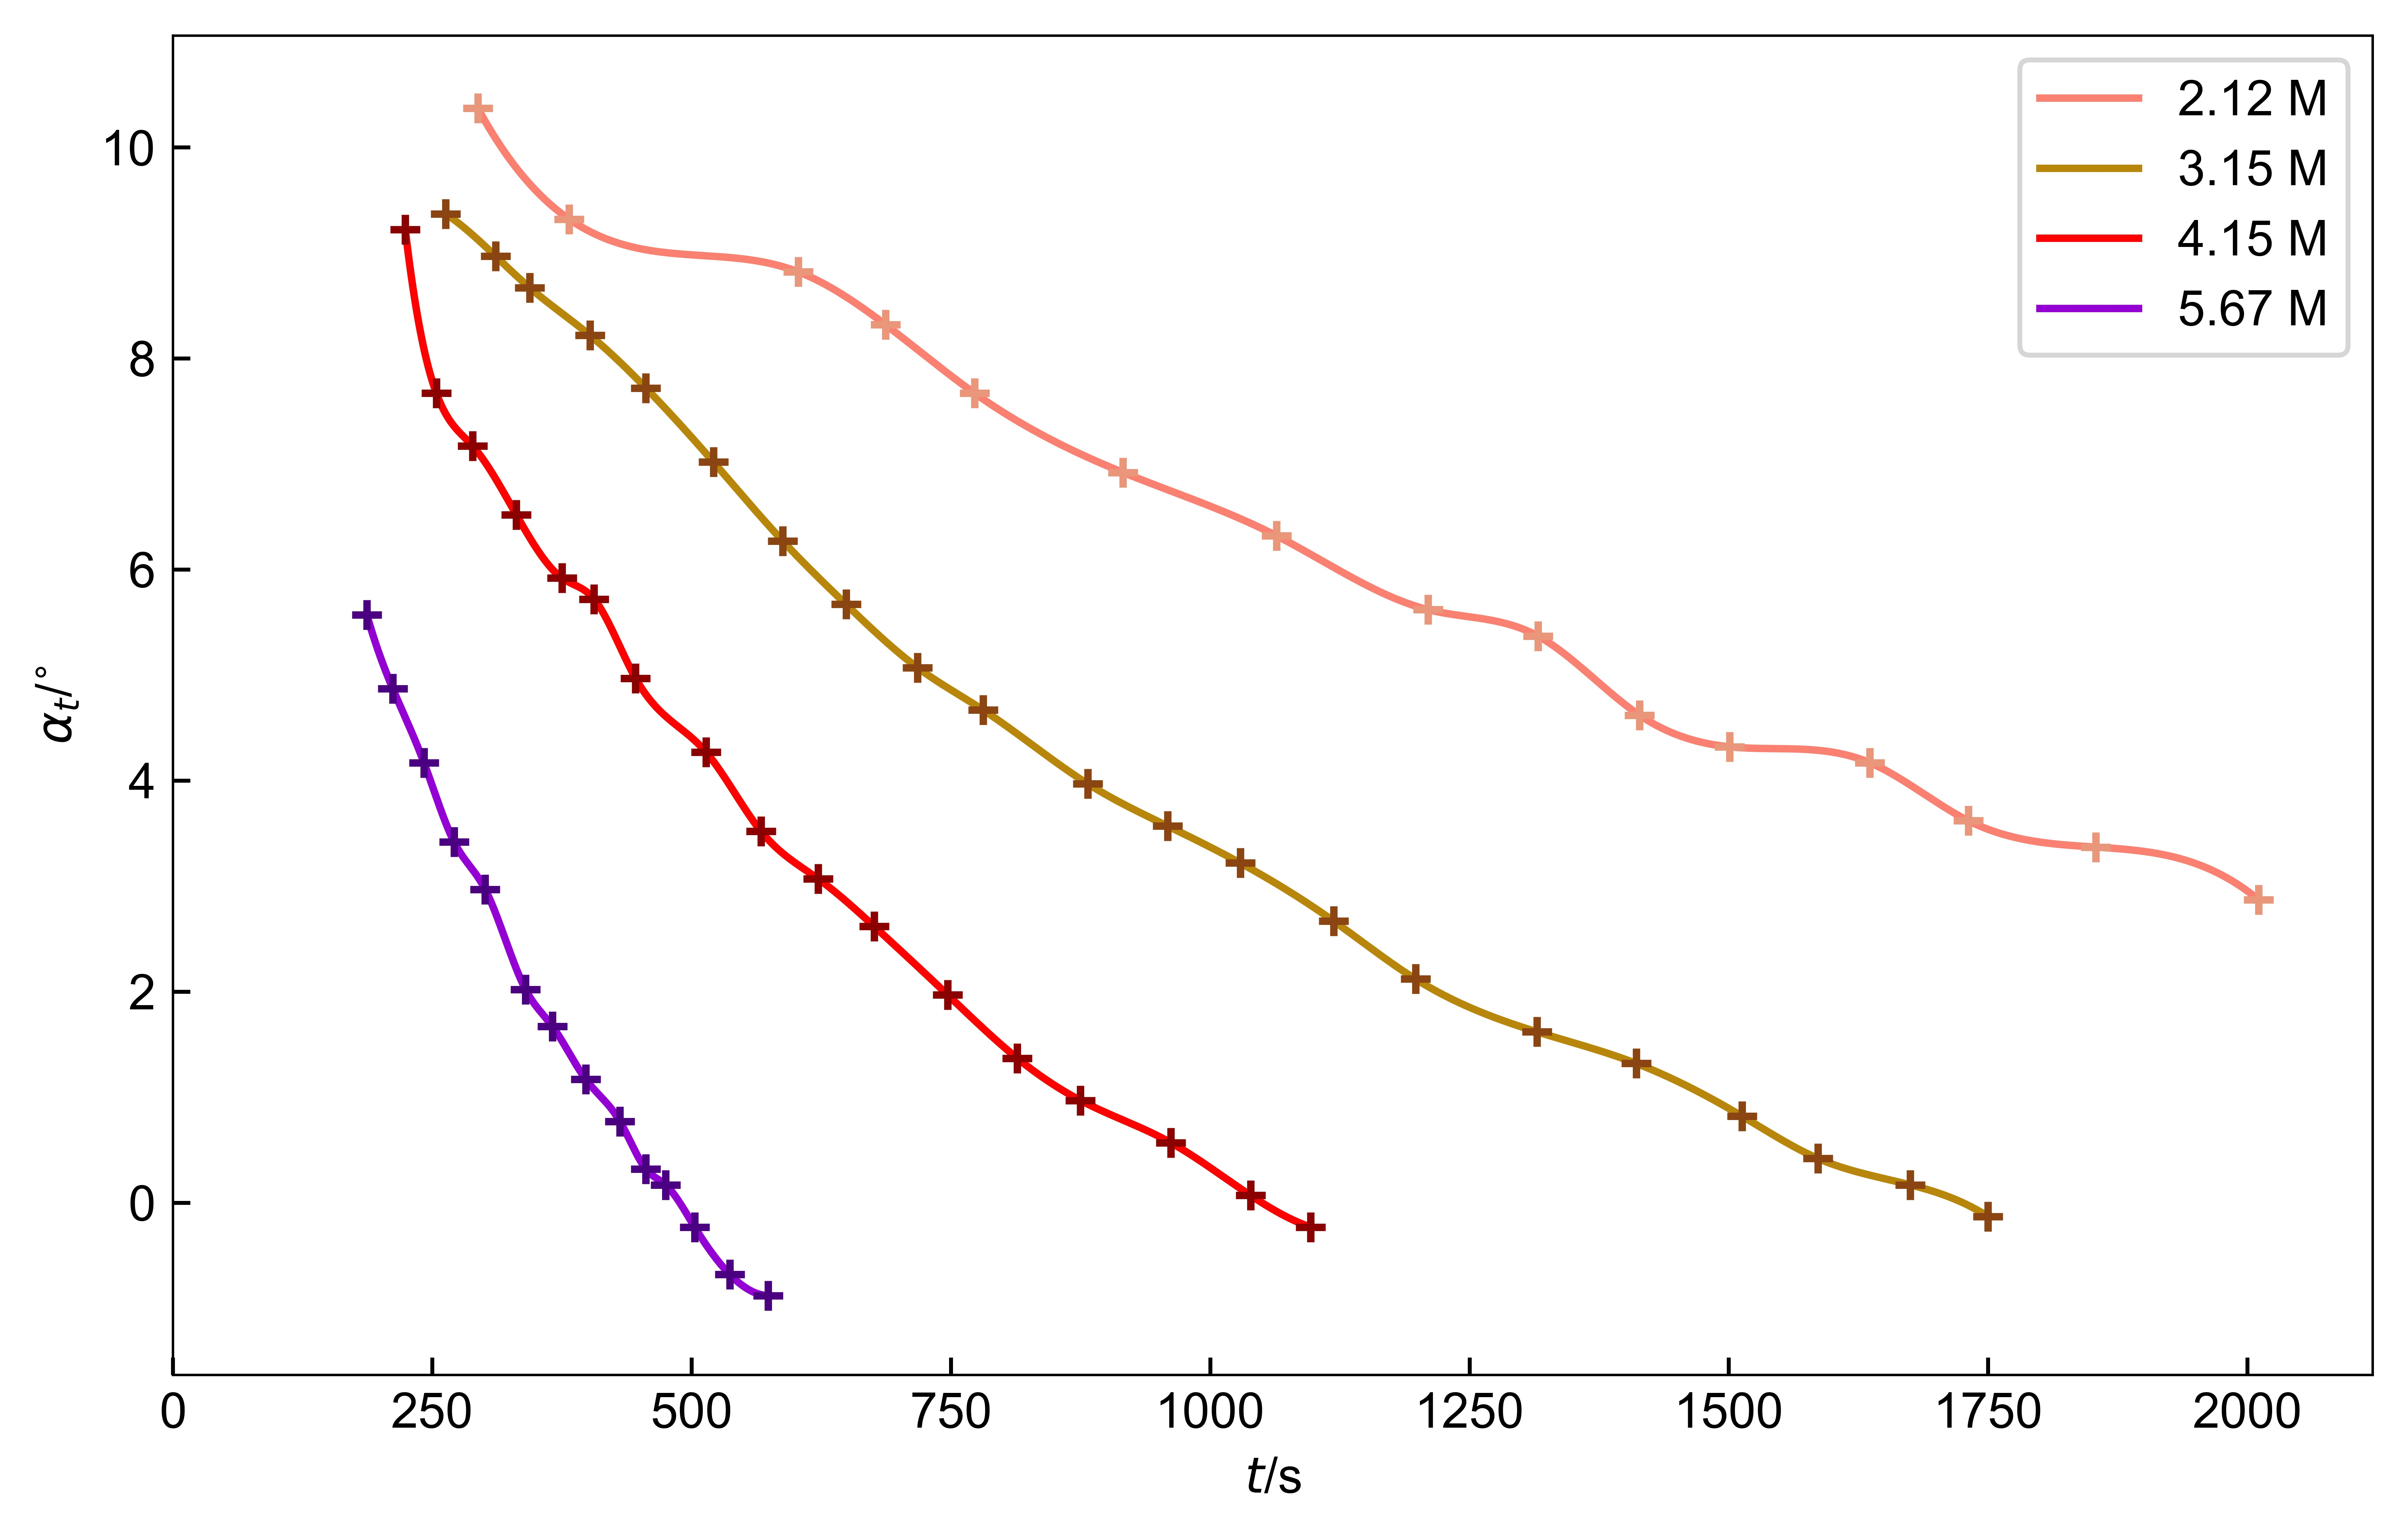
\includegraphics[width=0.8\textwidth]{1.jpg}
 	\bicaption{不同盐酸浓度下混合液$\alpha_{t}-t$图}{$\alpha_{t}-t$ diagram under different hydrochloric acid concentration}
 \end{figure}
 \par
 需要说明的是,上述盐酸浓度是加入的盐酸原溶液的浓度,混合液中实际的盐酸浓度是该浓度的一半。根据\textbf{图1}可以看出,同一时间$\alpha_{t}$随盐酸浓度增大而减小,即随着盐酸浓度升高,蔗糖转化反应速度加快。
\subsubsection{$(\alpha_{t}-\alpha_{\infty})$和${\rm lg}(\alpha_{t}-\alpha_{\infty})$数据}
根据\textbf{表2}数据和$\alpha_{\infty}=-4.03^{\circ}$,计算不同盐酸浓度下的$(\alpha_{t}-\alpha_{\infty})$和${\rm lg}(\alpha_{t}-\alpha_{\infty})$数据,记$\alpha_{\infty}-\alpha_{t}=\alpha_{1}$,各项数据示于\textbf{表4}。
 \begin{table}[h]
	\centering
	\zihao{5}
	\bicaption{不同盐酸浓度下混合液$(\alpha_{t}-\alpha_{\infty})$和${\rm lg}(\alpha_{t}-\alpha_{\infty})$数据}{Data of $(\alpha_{t}-\alpha_{\infty})$和${\rm lg}(\alpha_{t}-\alpha_{\infty})$ under different hydrochloric acid concentration}
	\begin{tabular}{ccccccccccccccc}
		\toprule
		\multicolumn{3}{c}{$c({\rm HCl})=2.12\ \ {\rm M}$} & & \multicolumn{3}{c}{$c({\rm HCl})=3.15\ \ {\rm M}$} & & \multicolumn{3}{c}{$c({\rm HCl})=4.15\ \ {\rm M}$} & & \multicolumn{3}{c}{$c({\rm HCl})=5.67\ \ {\rm M}$} \\
		\midrule
		$t/{\rm s}$ & $\alpha_{1}/^{\circ}$ & ${\rm lg}\alpha_{1}$ & &$t/{\rm s}$ & $\alpha_{1}/^{\circ}$ & ${\rm lg}\alpha_{1}$ & &$t/{\rm s}$ & $\alpha_{1}/^{\circ}$ & ${\rm lg}\alpha_{1}$ & &$t/{\rm s}$ & $\alpha_{1}/^{\circ}$ & ${\rm lg}\alpha_{1}$  \\
		\midrule
	294  & 14.40 & 1.158 &  & 263  & 13.40 & 1.127 &  & 224  & 13.25 & 1.122 &  & 187 & 9.60 & 0.982 \\
	382  & 13.35 & 1.125 &  & 311  & 13.00 & 1.114 &  & 254  & 11.70 & 1.068 &  & 212 & 8.90 & 0.949 \\
	603  & 12.85 & 1.109 &  & 344  & 12.70 & 1.104 &  & 289  & 11.20 & 1.049 &  & 242 & 8.20 & 0.914 \\
	687  & 12.35 & 1.092 &  & 402  & 12.25 & 1.088 &  & 331  & 10.55 & 1.023 &  & 271 & 7.45 & 0.872 \\
	773  & 11.70 & 1.068 &  & 456  & 11.75 & 1.070 &  & 375  & 9.95  & 0.998 &  & 301 & 7.00 & 0.845 \\
	916  & 10.95 & 1.039 &  & 521  & 11.05 & 1.043 &  & 406  & 9.75  & 0.989 &  & 340 & 6.05 & 0.782 \\
	1064 & 10.35 & 1.015 &  & 588  & 10.30 & 1.013 &  & 446  & 9.00  & 0.954 &  & 366 & 5.70 & 0.756 \\
	1210 & 9.65  & 0.985 &  & 649  & 9.70  & 0.987 &  & 514  & 8.30  & 0.919 &  & 398 & 5.20 & 0.716 \\
	1316 & 9.40  & 0.973 &  & 718  & 9.10  & 0.959 &  & 567  & 7.55  & 0.878 &  & 431 & 4.80 & 0.681 \\
	1414 & 8.65  & 0.937 &  & 781  & 8.70  & 0.940 &  & 622  & 7.10  & 0.851 &  & 456 & 4.35 & 0.638 \\
	1501 & 8.35  & 0.922 &  & 882  & 8.00  & 0.903 &  & 676  & 6.65  & 0.823 &  & 475 & 4.20 & 0.623 \\
	1636 & 8.20  & 0.914 &  & 959  & 7.60  & 0.881 &  & 747  & 6.00  & 0.778 &  & 503 & 3.80 & 0.580 \\
	1731 & 7.65  & 0.884 &  & 1029 & 7.25  & 0.860 &  & 814  & 5.40  & 0.732 &  & 537 & 3.35 & 0.525 \\
	1854 & 7.40  & 0.869 &  & 1119 & 6.70  & 0.826 &  & 875  & 5.00  & 0.699 &  & 574 & 3.15 & 0.498 \\
	2011 & 6.90  & 0.839 &  & 1198 & 6.15  & 0.789 &  & 962  & 4.60  & 0.663 &  &     &      &       \\
	&       &       &  & 1315 & 5.65  & 0.752 &  & 1039 & 4.10  & 0.613 &  &     &      &       \\
	&       &       &  & 1411 & 5.35  & 0.728 &  & 1097 & 3.80  & 0.580 &  &     &      &       \\
	&       &       &  & 1513 & 4.85  & 0.686 &  &      &       &       &  &     &      &       \\
	&       &       &  & 1586 & 4.45  & 0.648 &  &      &       &       &  &     &      &       \\
	&       &       &  & 1675 & 4.20  & 0.623 &  &      &       &       &  &     &      &       \\
	&       &       &  & 1750 & 3.90  & 0.591 &  &      &       &       &  &     &      &      \\
		
		
		\bottomrule
	\end{tabular}
\end{table}
\par 

\subsubsection{${\rm lg}(\alpha_{t}-\alpha_{\infty})-t$图与反应级数}
根据\textbf{表4}数据,作出不同盐酸浓度下混合液${\rm lg}(\alpha_{t}-\alpha_{\infty})-t$散点图,并用python SciPy lingress进行线性拟合,作出不同盐酸浓度下混合液${\rm lg}(\alpha_{t}-\alpha_{\infty})-t$拟合直线,如\textbf{图2}所示。

\begin{figure}[h]
	\centering
	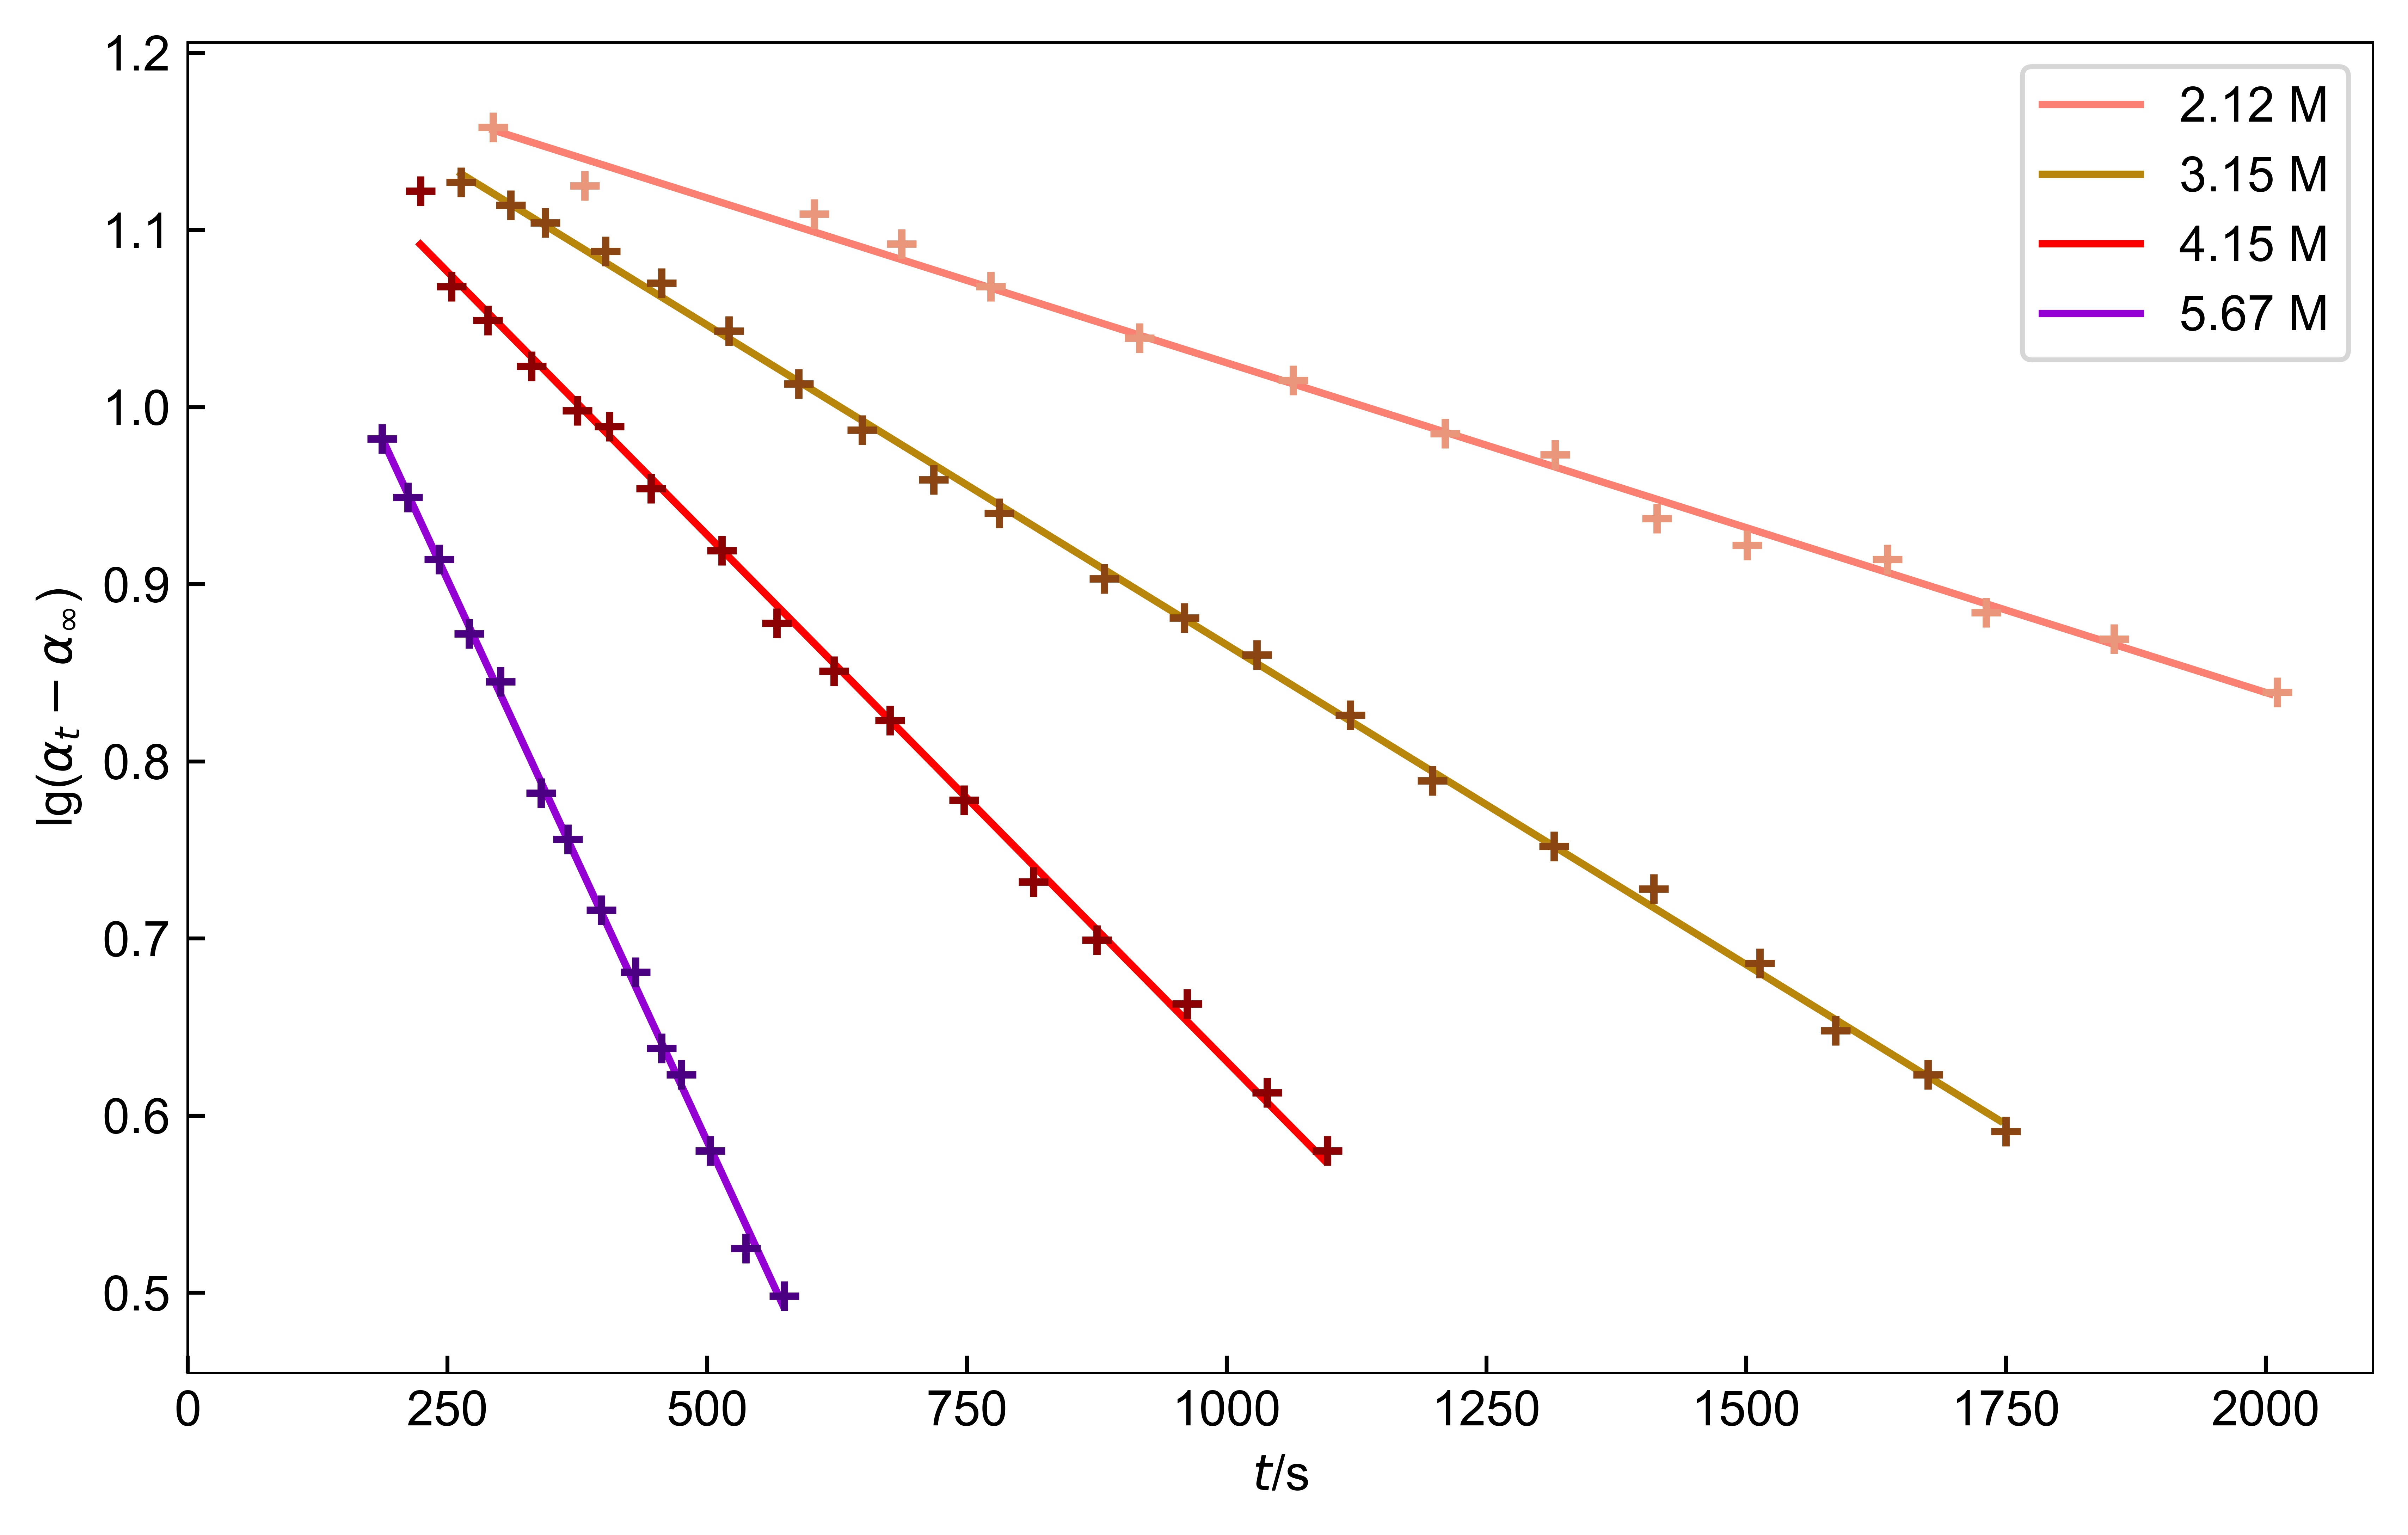
\includegraphics[width=0.8\textwidth]{2.jpg}
	\bicaption{不同盐酸浓度下混合液${\rm lg}(\alpha_{t}-\alpha_{\infty})-t$图}{${\rm lg}(\alpha_{t}-\alpha_{\infty})-t$ diagram under different hydrochloric acid concentration}
\end{figure}
\par
根据\textbf{图2}可以看出,不同盐酸浓度下${\rm lg}(\alpha_{t}-\alpha_{\infty})-t$都具有良好的线性关系,根据一级反应的动力学特征
$$
{\rm ln}\frac{c_{0}}{c_{t}}=kt
$$
可以判断$\rm H^{+}$浓度固定的条件下,蔗糖转化反应为一级反应。$2.12\ \ {\rm M}$、$3.15\ \ {\rm M}$、$4.15\ \ {\rm M}$、$5.67\ \ {\rm M}$盐酸浓度下的回归直线方程分别为

$$
{\rm lg}(\alpha_{t}-\alpha_{\infty})-t=-1.861\times10^{-4}t/s+1.211,\ \ R=-0.9973
$$
$$
{\rm lg}(\alpha_{t}-\alpha_{\infty})-t=-3.610\times10^{-4}t/s+1.227,\ \ R=-0.9995
$$
$$
{\rm lg}(\alpha_{t}-\alpha_{\infty})-t=-5.944\times10^{-4}t/s+1.225,\ \ R=-0.9983
$$
$$
{\rm lg}(\alpha_{t}-\alpha_{\infty})-t=-1.269\times10^{-3}t/s+1.220,\ \ R=-0.9993
$$
\subsubsection{反应速率常数$k$和半衰期$t_{1/2}$}
根据
$$
{\rm lg}(\alpha_{t}-\alpha_{\infty})=-\frac{k}{2.303}t+{\rm lg}(\alpha_{0}-\alpha_{\infty})
$$
可以用拟合直线的斜率$a$计算速率常数$k$,即
$$
k=-2.303a
$$
根据线性回归分析的相关知识,拟合直线斜率的标准差
$$
\sigma_{a}=|a|\sqrt{\frac{\frac{1}{R^{2}}-1}{n-2}}
$$
其中a为回归直线的斜率,R为回归直线的相关系数,n为测量次数即数据点的个数。根据以上公式,分别计算$2.12\ \ {\rm M}$、$3.15\ \ {\rm M}$、$4.15\ \ {\rm M}$、$5.67\ \ {\rm M}$盐酸浓度下回归直线斜率的标准差
$$
\sigma_{a,\ \ {\rm 2.12 M}}=1.861\times10^{-4}\times\sqrt{\frac{0.9973^{-2}-1}{15-2}}\ \ {\rm s^{-1}}=0.04\times10^{-4}\ \ {\rm s^{-1}}
$$
$$
\sigma_{a,\ \ {\rm 3.15 M}}=3.610\times10^{-4}\times\sqrt{\frac{0.9995^{-2}-1}{21-2}}\ \ {\rm s^{-1}}=0.03\times10^{-4}\ \ {\rm s^{-1}}
$$
$$
\sigma_{a,\ \ {\rm 4.15 M}}=5.944\times10^{-4}\times\sqrt{\frac{0.9983^{-2}-1}{17-2}}\ \ {\rm s^{-1}}=0.09\times10^{-4}\ \ {\rm s^{-1}}
$$
$$
\sigma_{a,\ \ {\rm 5.67 M}}=12.69\times10^{-4}\times\sqrt{\frac{0.9993^{-2}-1}{14-2}}\ \ {\rm s^{-1}}=0.14\times10^{-4}\ \ {\rm s^{-1}}
$$
速率常数的标准差
$$
\sigma_{k}=2.303\sigma_{a}
$$
一级反应的半衰期满足
$$
t_{1/2}=\frac{0.693}{k}
$$
半衰期的标准差
$$
\sigma_{t_{1/2}}=0.693\frac{\sigma_{k}}{k^{2}}
$$
根据拟合直线方程,计算不同盐酸浓度下的反应速率常数$k$、半衰期$t_{1/2}$及各自的标准差$\sigma_{k}$、$\sigma_{t_{1/2}}$,结果示于\textbf{表5},其中$c({\rm HCl})$是加入盐酸的浓度,$a$是拟合直线的斜率。
\begin{table}[h]
	\centering
	\zihao{5}
	\bicaption{不同盐酸浓度下$k$与$t_{1/2}$计算结果}{Calculation results of $k$ and $t_{1/2}$ under different hydrochloric acid concentrations}
	\begin{tabular}{cccc}
		\toprule

		$c({\rm HCl}) / {\rm M}$ & $a/{\rm 10^{-4} \ \ s^{-1}}$ & $k/{\rm 10^{-4} \ \ s^{-1}}$ & $t_{1/2} /{\rm s}$\\
		\midrule
		2.12 & $-1.86\pm 0.04$ &  $4.28\pm 0.09$ & $1617\pm 35$ \\
		3.15 & $-3.61\pm 0.03$ &  $8.31\pm 0.07$ & $834\pm 7$ \\
		4.15 & $-5.94\pm 0.09$ & $13.7\pm 0.2$ & $506\pm 8$ \\
		5.67 & $-12.7\pm 0.1$ & $29.2\pm 0.3$ & $237\pm 3$ \\
		
		\bottomrule
	\end{tabular}
\end{table}
\par
\subsubsection{H$^{+}$的反应级数}
考虑H$^{+}$对反应速率的影响,有
$$
k=k_{0}+k_{\rm H^{+}}c^{n}_{\rm H^{+}}
$$
其中$k_{0}$是$c_{\rm H^{+}}\rightarrow0$时的反应速率常数,$k_{\rm H^{+}}$为酸催化速率常数,$k$为表观速率常数,$n$为$\rm H^{+}$的反应级数。两边取以$10$为底的对数,即得
$$
{\rm lg}(k-k_{0})=n{\rm lg}c_{\rm H^{+}}+{\rm lg}k_{\rm H^{+}}
$$
故作出${\rm lg}(k-k_{0})-{\rm lg}c_{\rm H^{+}}$拟合直线,由直线斜率即可求出$\rm H^{+}$的反应级数$n$。\par 
首先用曲线外推求出$k_{0}$。根据\textbf{表5}数据,考虑到$c_{\rm H^{+}}=\frac{1}{2}c({\rm HCl})$,用python SciPy库2次样条插值曲线拟合,作出$k-c_{\rm HCl}$曲线图,如\textbf{图3}所示。
\begin{figure}[h]
	\centering
	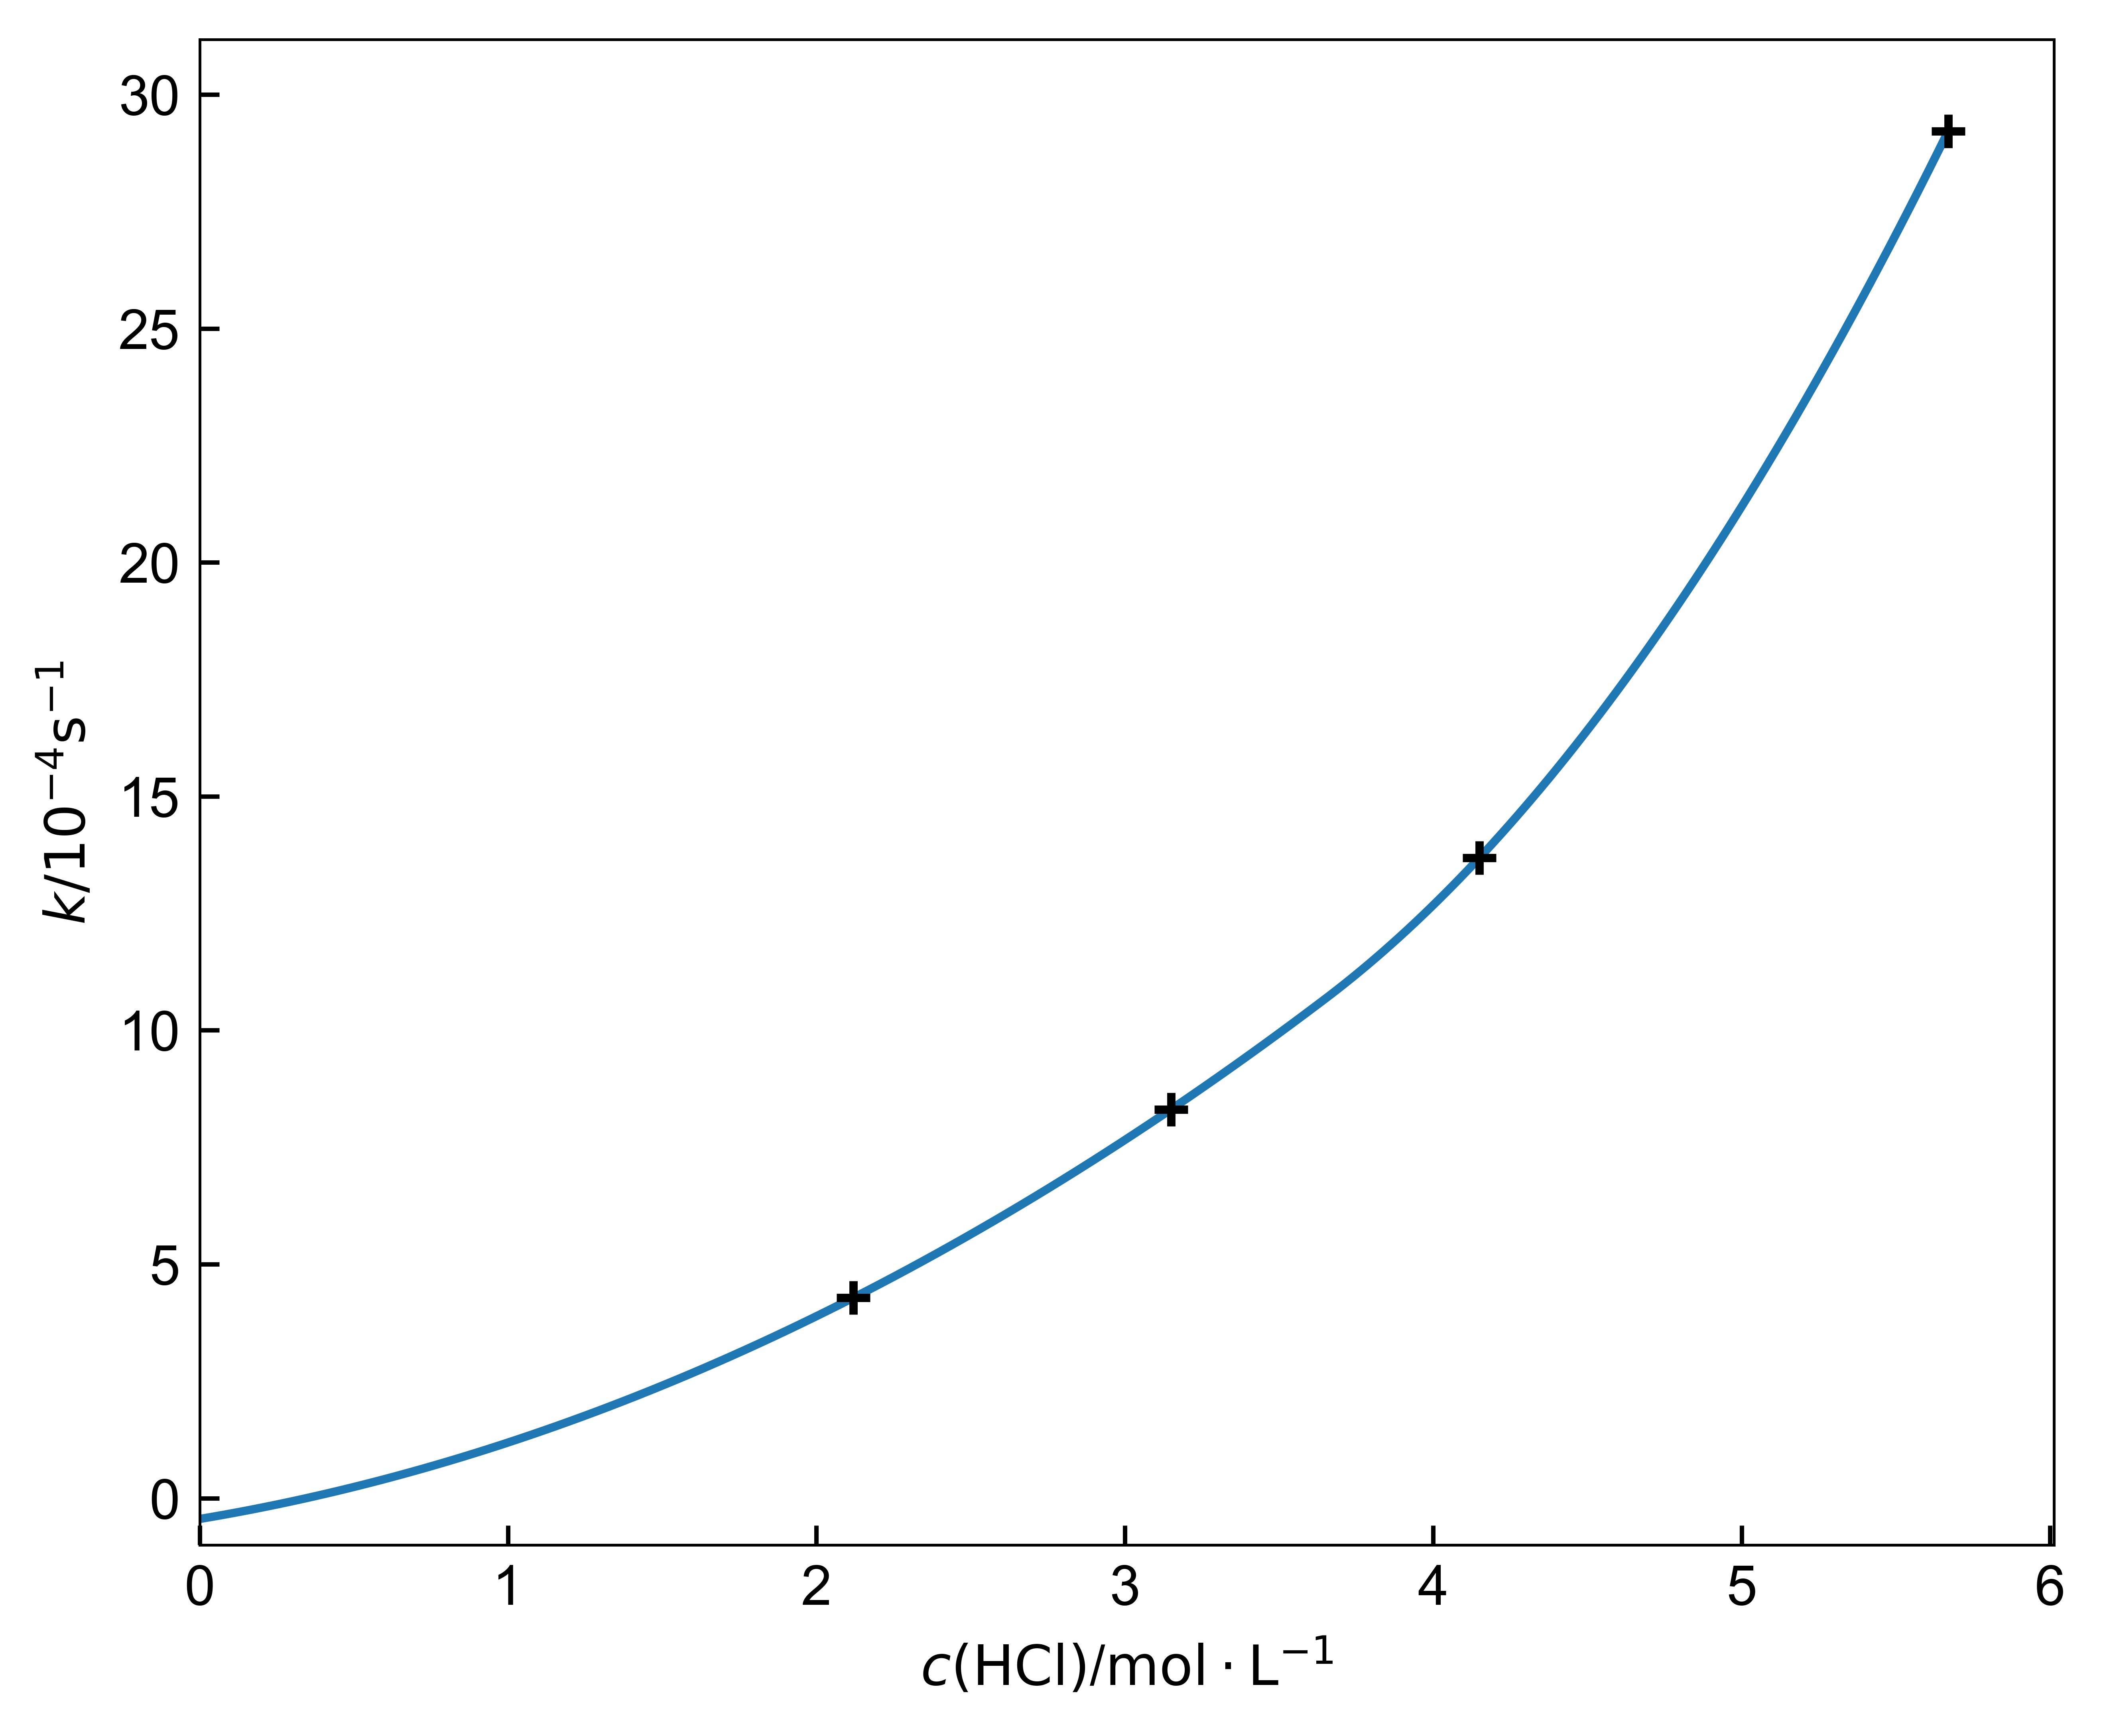
\includegraphics[width=0.55\textwidth]{3.jpg}
	\bicaption{$k-c_{\rm HCl}$曲线}{$k-c_{\rm HCl}$ diagram}
\end{figure}
\par
外推得到$c({\rm HCl})=0$时,$k_{0}=-0.444\times10^{-4}\ \ {\rm s^{-1}}$。考虑到实际在没有$\rm H^{+}$作为催化剂时,蔗糖的水解速率极慢,几乎可以忽略不计,因此实际的$k_{0}$值很小,几乎为0。虽然曲线外推得到的$k_{0}$为明显不合理的负值,但由于所得$k_{0}$的绝对值很小,非常接近0,与实际相符,因此基本可以认为误差不大。\par 
根据求得的$k_{0}=-0.444\times10^{-4}\ \ {\rm s^{-1}}$和\textbf{表5}数据,计算$c_{\rm H^{+}}=\frac{1}{2}c({\rm HCl})$,${\rm lg}c_{\rm H^{+}}$与${\rm lg}(k-k_{0})$,计算结果示于\textbf{表6}。
\begin{table}[h]
	\centering
	\zihao{5}
	\bicaption{$c_{\rm H^{+}}$,${\rm lg}c_{\rm H^{+}}$与${\rm lg}(k-k_{0})$计算结果}{Calculation results of $c_{\rm H^{+}}$, ${\rm lg}c_{\rm H^{+}}$ and ${\rm lg}(k-k_{0})$ }
	\begin{tabular}{cccc}
		\toprule
		
		$c_{\rm H^{+}} / {\rm M}$ & ${\rm lg}c_{\rm H^{+}}$ & $(k-k_{0})/{\rm 10^{-4} \ \ s^{-1}}$ & ${\rm lg}(k-k_{0})$\\
		\midrule
		1.06 & 0.0253 &  4.729 & 0.6748 \\
		1.58 & 0.1973 &  8.756 &  0.9423\\
		2.08 & 0.3170 & 14.133 & 1.1502 \\
		2.84 & 0.4526 & 29.664 & 1.4722 \\
		\bottomrule
	\end{tabular}
\end{table}
\par
根据\textbf{表6}数据,作出${\rm lg}c_{\rm H^{+}}-{\rm lg}(k-k_{0})$散点图,并用python SciPy lingress进行线性拟合,作出${\rm lg}c_{\rm H^{+}}-{\rm lg}(k-k_{0})$拟合直线,如\textbf{图4}所示。
\begin{figure}[h]
	\centering
	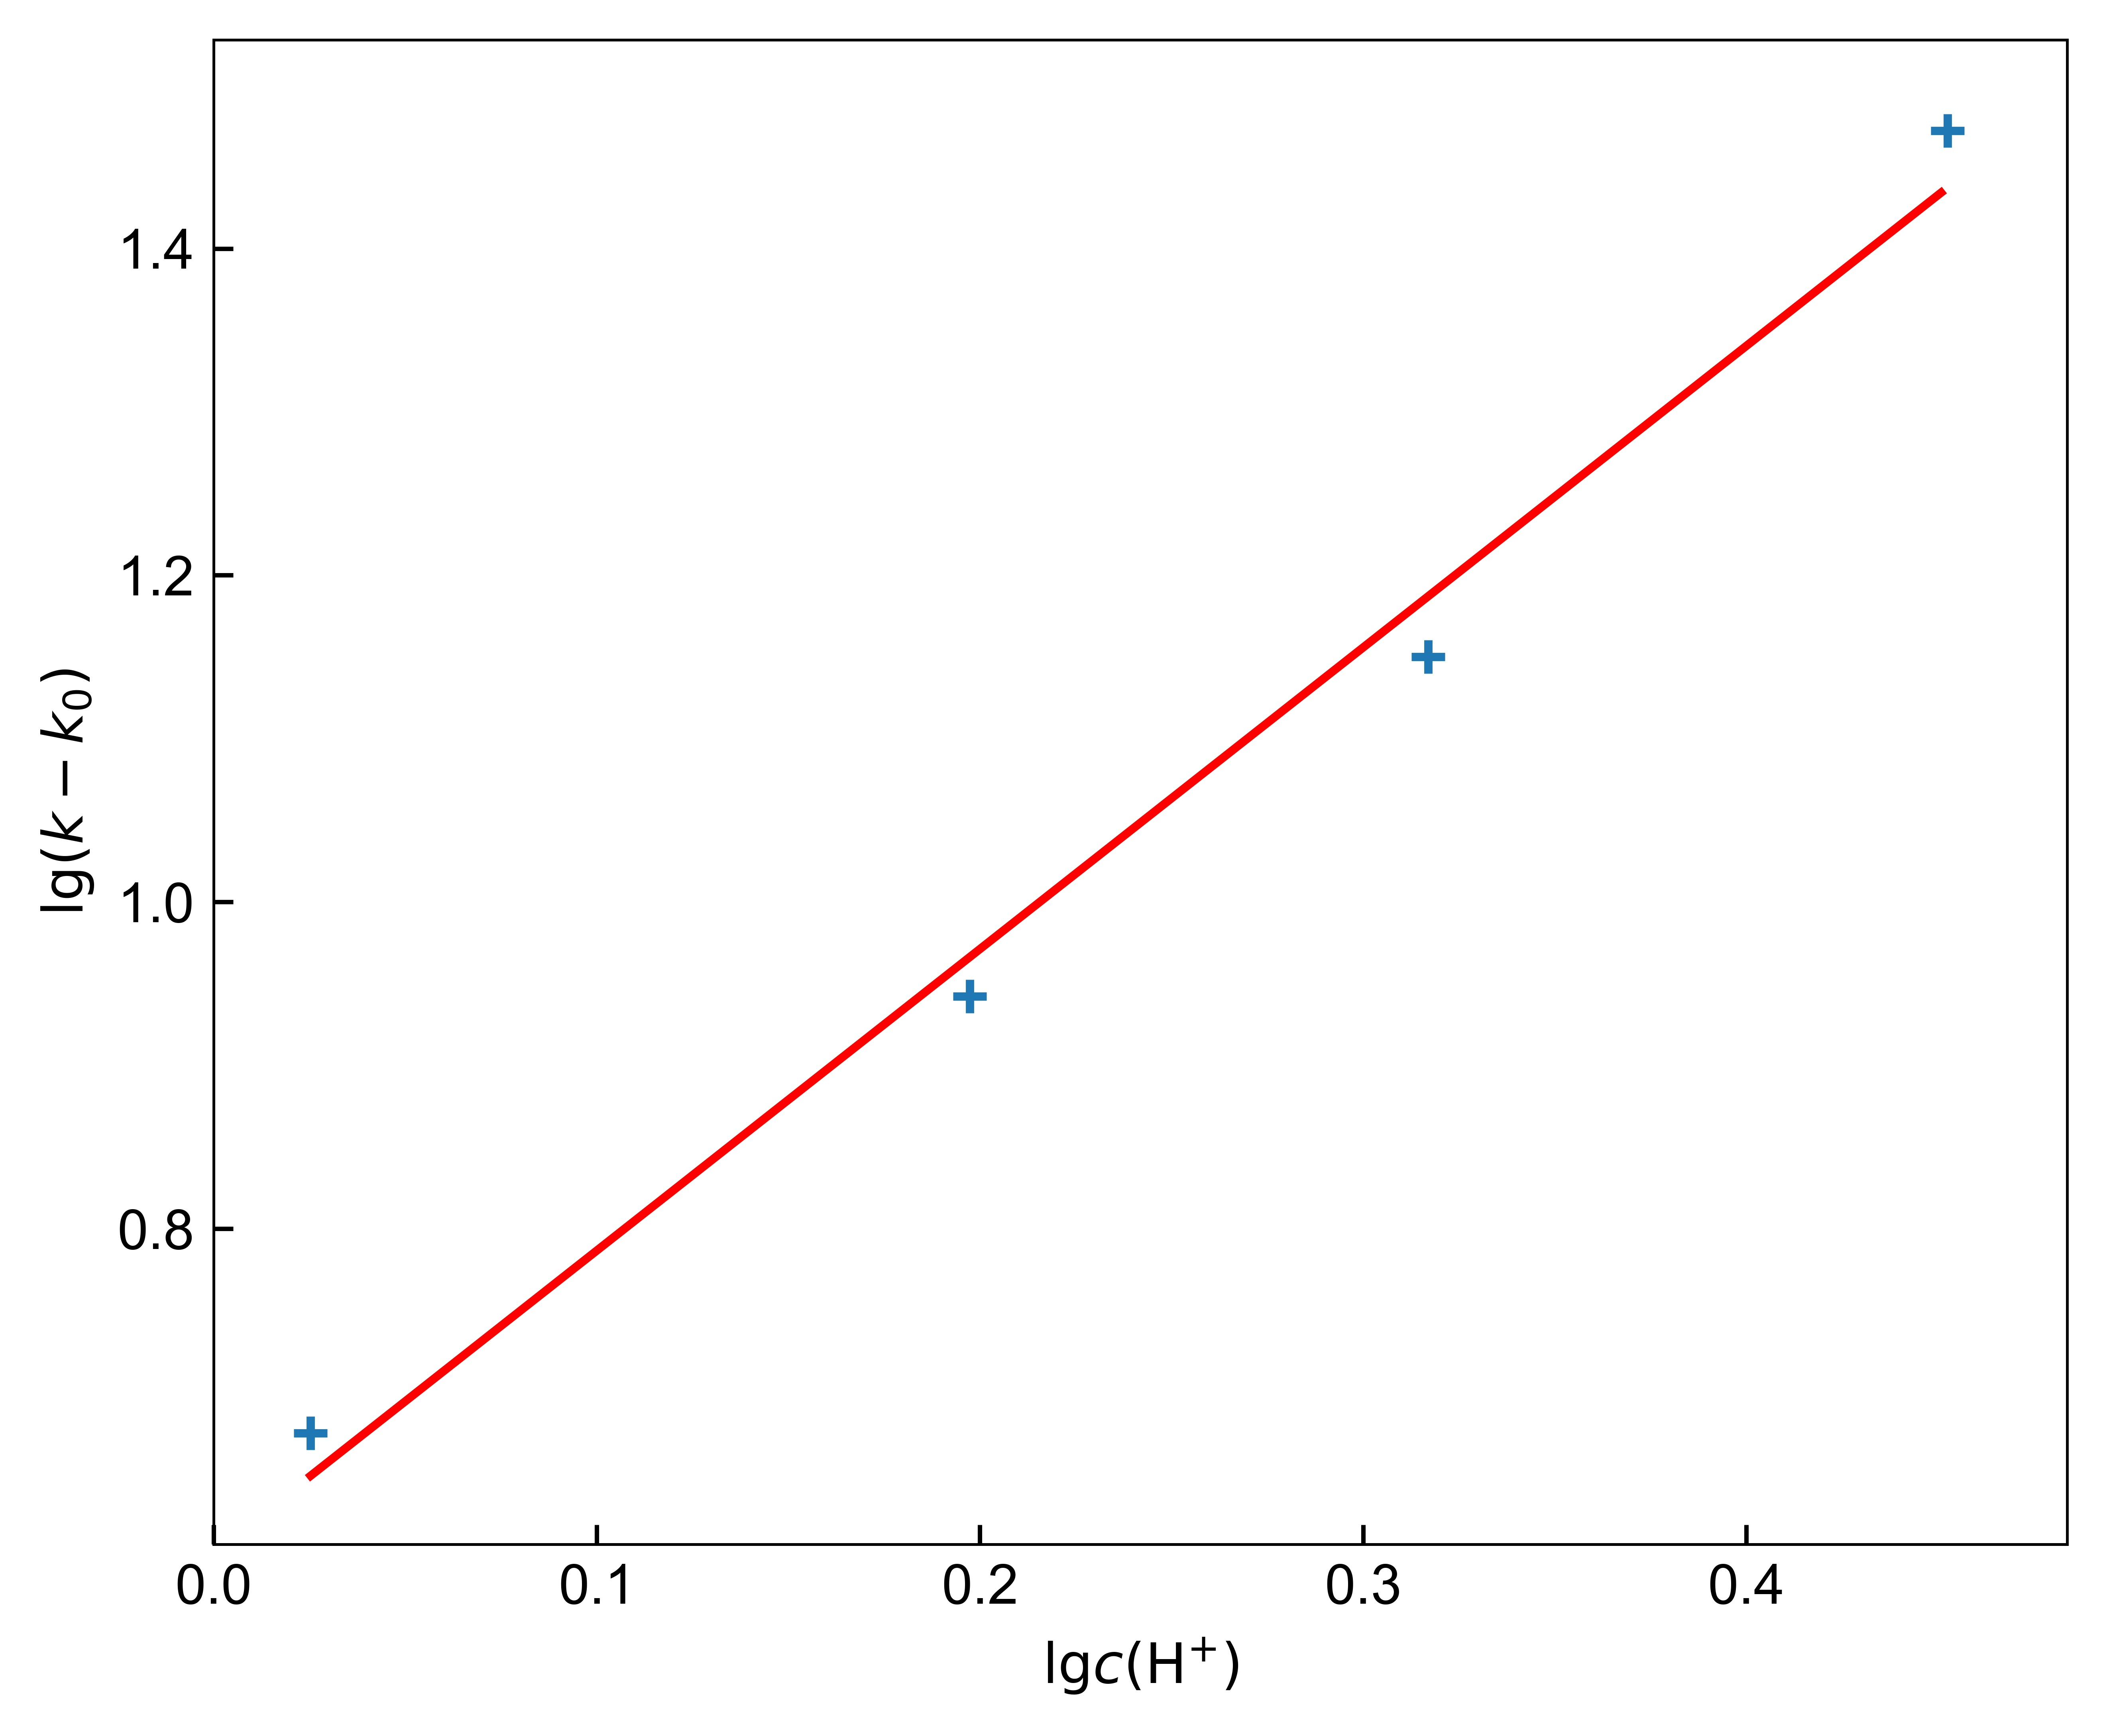
\includegraphics[width=0.6\textwidth]{4.jpg}
	\bicaption{${\rm lg}c_{\rm H^{+}}-{\rm lg}(k-k_{0})$图}{${\rm lg}c_{\rm H^{+}}-{\rm lg}(k-k_{0})$ diagram}
\end{figure}
\par
根据\textbf{图4}可以看出,${\rm lg}c_{\rm H^{+}}-{\rm lg}(k-k_{0})$具有良好的线性关系,回归直线方程为
$$
{\rm lg}(k-k_{0})=1.8455\ \ {\rm lg}c_{\rm H^{+}}+0.6021,\ \ R=0.9944
$$
故$\rm H^{+}$的反应级数
$$
n=1.8455\approx2
$$

 	 \section{讨论与结论}
		\subsection{实验讨论}
 			\subsubsection{旋光角未由右旋变为左旋即停止测量的影响}
如3.1.2所述,在测定$5.67\ \ {\rm M}$盐酸溶液与蔗糖溶液混合液的旋光度时,因疏忽未等旋光角由右旋变为左旋即停止测量。该操作失误对测量结果是否造成了影响?经分析,由于该组实验已经获取了超过12组有效数据,且考虑到旋光角接近由右旋变为左旋时测量误差相对较大,故该失误对反应速率常数$k$和半衰期$t_{1/2}$计算结果的影响较小;实际上,如果仅考虑获取足够的有效实验数据,并不需要测至旋光角由右旋变为左旋;要求每组测至旋光角变为左旋,主要目的是使得旋光度测量的时间具有可比性,即通过测量不同盐酸浓度下混合液旋光角发生变化所用的时间,可以大致估测蔗糖转化反应的速率和半衰期,从而对于蔗糖转化反应的动力学特征建立直观的印象,初步检验实验结果是否正确。因此,虽然等旋光角由右旋变为左旋后再停止测量的操作对实验结果的准确度影响不大,但对于整个实验过程而言仍然具有重要的意义。
 	 	\subsubsection{误差来源分析与实验改进}
本次实验的误差主要来自两方面:\par 
第一,人眼判断旋光仪读数位置不精确带来的误差。在实际测量过程中,需要手动调节旋光仪度盘调节手轮至三分视场消失、视野暗度相同,但每一次人眼判断暗视场出现的位置有所不同,从而引入了人为误差。\par 
第二,反应体系恒温不够充分完全、反应在不同温度下进行带来的误差。根据Arrhenius公式$k=Ae^{-\frac{E_{a}}{RT}}$,化学反应速率常数$k$对温度十分敏感,较小的温度改变即可导致反应速率的很大变化;在实验过程中,向蔗糖溶液中加入盐酸溶液、摇匀、润洗旋光管的操作在室温下进行,未对反应体系加以保温,可能导致该时间段内反应速率产生较大变化,从而对$k$和$t_{1/2}$的测定引入误差。\par 
为减小以上两方面误差,首先可以用监视设备实现旋光仪读数位置的自动判断,避免人为误差;其次需要尽量缩短加入盐酸溶液、摇匀、润洗旋光管所需时间,各项操作尽可能在恒温水浴中进行。


 	 \subsection{实验结论}
本实验使用目视旋光仪测定蔗糖转化过程中体系的旋光度,依次测量了加入盐酸浓度分别为$5.67\ \ {\rm M}$、$2.12 \ \ {\rm M}$、$3.15\ \ {\rm M}$、$4.15\ \ {\rm M}$、$5.67\ \ {\rm M}$时的体系旋光度$\alpha_{t}$随时间$t$的变化,验证了蔗糖转化反应对蔗糖是一级反应,作出了不同盐酸浓度下混合液$\alpha_{t}-t$图和${\rm lg}(\alpha_{t}-\alpha_{\infty})-t$图,测定了加入盐酸浓度分别为$2.12\ \ {\rm M}$、$3.15\ \ {\rm M}$、$4.15\ \ {\rm M}$、$5.67\ \ {\rm M}$时,反应速率常数$k$分别为$(4.28\pm 0.09)\times10^{-4}\ \ s^{-1}$、$(8.31\pm 0.07)\times10^{-4}\ \ s^{-1}$、$(13.7\pm 0.2)\times10^{-4}\ \ s^{-1}$、$(29.2\pm 0.3)\times10^{-4}\ \ s^{-1}$,计算了对应的半衰期$t_{1/2}$分别为$(1617\pm 35)\ \ {\rm s}$、$(834\pm 7)\ \ {\rm s}$、$(506\pm 8)\ \ {\rm s}$、$(237\pm 3) \ \ {\rm s}$,并得到了$\rm H^{+}$的反应级数$\rm n\approx2$。\par 
本次实验巧妙地把蔗糖转化反应的程度转换为体系的旋光度,通过测量蔗糖转化反应的初速率得到了不同盐酸浓度下的反应速率常数、反应级数和半衰期,从而更加深入地理解了一级反应的动力学特征。

 

   
\vbox{}
\vbox{}

\bibliographystyle{achemso}
\bibliography{cite}



\end{document}